\documentclass[conference]{IEEEtran}
\IEEEoverridecommandlockouts

\usepackage{cite}
\usepackage{amsmath,amssymb,amsfonts,amsthm}
\usepackage{booktabs}
\usepackage{graphicx}
\usepackage{textcomp}
\usepackage{xcolor}
\usepackage{listings}
\usepackage{url}
\let\labelindent\relax
\usepackage{enumitem}
\setlist[itemize]{leftmargin=*, topsep=1pt, itemsep=0pt, parsep=0pt}

\newlength{\ieeeindent}
\setlength{\ieeeindent}{1em}
\newcommand{\parhead}[1]{\par\noindent\hspace*{\ieeeindent}\textbf{#1}}

\makeatletter
\newtheoremstyle{ieeeitalic}
  {1.5pt}
  {1.5pt}
  {\itshape}
  {\ieeeindent}
  {\bfseries\itshape}
  {:}
  {0.4em}
  {\thmname{#1}\thmnumber{ #2}\thmnote{ (#3)}}
\theoremstyle{ieeeitalic}
\newtheorem{proposition}{Proposition}

\renewenvironment{proof}[1][\proofname]{\par
  \pushQED{\qed}%
  \normalfont\topsep1.5pt plus 1pt\relax
  \trivlist
  \item[\hskip\labelsep\hspace*{\ieeeindent}\itshape #1:]\ignorespaces
}{%
  \popQED\endtrivlist\@endpefalse
}
\makeatother

\newcommand{\GS}{\mathrm{GS}}
\newcommand{\dhatmax}{\hat{d}_{\max}}
\newcommand{\Lap}{\mathrm{Lap}}
\newcommand{\RE}{\mathrm{RE}}
\newcommand{\DeriveGS}{\mathsf{DeriveGS}}
\newcommand{\VerifyCert}{\mathsf{VerifyCert}}
\newcommand{\Proj}{\mathsf{Proj}}

\lstdefinestyle{dslstyle}{
  basicstyle=\ttfamily\scriptsize,
  columns=flexible,
  keepspaces=true,
  frame=single,
  rulecolor=\color{black!55},
  framesep=2pt,
  xleftmargin=2pt,
  xrightmargin=2pt,
  aboveskip=2pt,
  belowskip=2pt,
  morekeywords={return,for,in,aggregate,project,size,comb,sum,clip,min,max,pow},
  keywordstyle=\bfseries,
  morecomment=[l]{\#},
  commentstyle=\rmfamily\itshape\color{black!65}
}

\begin{document}
\bstctlcite{IEEEexample:BSTcontrol}

\title{CertiCount: Verifier-Guided Program Synthesis and Certified Execution for Substructure Counting under Local Differential Privacy}

\author{\IEEEauthorblockN{Anonymous Authors}
\IEEEauthorblockA{Affiliation Placeholder\\
Email: placeholder@domain.org}}

\maketitle

\begin{abstract}
Large language models (LLMs) offer a natural-language interface for graph analytics, but counting substructures over sensitive user connections requires edge local differential privacy (edge-LDP) against an untrusted server. Delegating rule design and local counting to multi-agent LLMs is flawed: node LLMs miscount combinatorial patterns, prompt-serialized edge lists overflow context windows, noise calibrated to an ideal rule's global sensitivity ($\GS$) does not protect erratic LLM outputs, and unverified curator rules preclude safe extensibility. We propose \textsc{CertiCount}, a verifier-guided program synthesis and certified execution framework that decouples query design from private execution under $\varepsilon$-edge LDP. Using only public metadata, an untrusted curator LLM synthesizes estimators in a restricted graph-LDP domain-specific language (DSL), repaired by deterministic checker diagnostics. \textsc{CertiCount} statically derives $\GS$ via abstract interpretation, filters statistically degenerate estimators by noise-aware simulation on synthetic graphs, and issues sensitivity certificates that each node re-derives before deterministic local execution without LLM calls. Experiments on six real-world datasets show that \textsc{CertiCount} substantially outperforms multi-agent LLM baselines in accuracy and scalability, matches hand-crafted expert estimators on $k$-star queries and stays within $1.8\times$ of them on all other queries, and eliminates empirical sensitivity violations, while diagnostic repair improves publishable program yield at lower LLM call cost and generalizes to unseen subgraph queries.
\end{abstract}

\begin{IEEEkeywords}
local differential privacy, graph substructure counting, program synthesis, sensitivity analysis, large language models
\end{IEEEkeywords}

\section{Introduction}
\label{sec:intro}

Counting small graph substructures---such as node degrees, $k$-stars, wedges, and triangles---is fundamental to characterizing connectivity, clustering, and interaction patterns across social, communication, and biological networks~\cite{imola2021locally,he2025robust}. With large language models (LLMs) as natural-language interfaces~\cite{wang2023can,chen2024graphwiz}, analysts seek to pose ad-hoc graph queries without engineering algorithms per task. Yet edges encode confidential relationships, so edge local differential privacy ($\varepsilon$-edge LDP)~\cite{imola2021locally,imola2022communication} keeps each neighbor list local and perturbs all outgoing messages. Such analytics is inherently a \emph{multi-party cooperative} computation: an analyst poses the query, a curator designs the estimator, an aggregator combines reports, and many data owners compute locally---yet no party may see raw edges, and no party can trust the others' code or claims.

Existing paradigms trade extensibility against trustworthiness. Classical $\varepsilon$-edge LDP protocols~\cite{imola2021locally,imola2022communication,he2025robust,guo2025nam} achieve high utility via degree bounding and bias-corrected edge releases, yet require experts to derive unbiased estimators and global sensitivity ($\GS$) bounds per pattern. Multi-agent LLM frameworks such as PSC~\cite{zhang2026psc} automate counting with an untrusted curator LLM that formulates rules, a controller that splits $\varepsilon = \varepsilon_1 + \varepsilon_2 + \varepsilon_3$, and node LLM agents that count local patterns over private neighbor lists before adding $\Lap(\GS/\varepsilon_3)$ noise. Placing LLMs in rule formulation and private execution, however, raises three challenges:
\begin{itemize}
    \item \textbf{Unreliable counting and context bottlenecks.} LLMs miscount over long contexts~\cite{liu2023lost}, and serializing neighbor lists and dense randomized-response (RR) noisy edges overflows context windows as graphs scale~\cite{zhang2026psc}.
    \item \textbf{Invalidated privacy under black-box execution.} $\Lap(\GS/\varepsilon_3)$ noise guarantees $\varepsilon_3$-edge LDP only if the pre-noise mapping has sensitivity at most $\GS$~\cite{dwork2014algorithmic}, which erratic node LLM outputs break.
    \item \textbf{Untrusted synthesis and statistical degeneracy.} The curator's logic or claimed $\GS$ may be wrong, risking silent privacy violations; even privacy-valid programs degenerate if they apply non-linear combinatorics to RR rows without bias correction.
\end{itemize}

To address these challenges, we propose \textsc{CertiCount} (Fig.~\ref{fig:arch}), a verifier-guided synthesis and certified execution framework built on a strict separation of duties: \emph{the LLM designs, the system certifies, and nodes execute code}. Working offline on public metadata (query description and node count $n$), an untrusted curator LLM writes candidate estimators in a restricted graph-LDP domain-specific language (DSL). Building on established edge-LDP primitives---RR releases, per-node edge clipping~\cite{imola2022communication}, and unbiased noisy adjacency matrices (NAM-DPRD)~\cite{guo2025nam}---\textsc{CertiCount} repairs drafts with deterministic syntax, sensitivity, semantic, and small-graph falsification checkers. A static analyzer ($\DeriveGS$) derives $\GS$ bounds via abstract interpretation, zero-budget simulation on public synthetic graphs~\cite{holme2002growing,chung2002connected} filters degenerate estimators, and each node re-derives the sensitivity certificate ($\VerifyCert$) before deterministic local execution. The certified program thus acts as a machine-checkable contract between mutually distrusting parties, and the checker diagnostics turn LLM--verifier interaction into a cooperative design loop. Our contributions are:
\begin{itemize}
    \item \textbf{Decoupled Synthesis and Execution:} Nodes run certified DSL programs in a deterministic interpreter with zero node LLM calls, eliminating counting errors and context bottlenecks under $\varepsilon$-edge LDP.
    \item \textbf{Node-Verifiable Certification and Noise-Aware Selection:} A restricted graph-LDP DSL with abstract-interpretation $\GS$ derivation, node-side certificate re-derivation, and zero-budget simulation that filters privacy-valid yet statistically degenerate estimators.
    \item \textbf{Verifier-Guided Repair and Validation:} Stage-specific checker diagnostics drive within-session synthesis; on six real-world datasets, \textsc{CertiCount} approaches expert estimators, prevents sensitivity violations, improves publishable yield at lower LLM cost, and generalizes to unseen queries.
\end{itemize}

\section{Related Work}
\label{sec:related}

\parhead{Edge-LDP Graph Substructure Counting.}
Unlike centralized graph DP~\cite{dwork2014algorithmic}, $\varepsilon$-edge LDP perturbs adjacency lists locally at each user. To reduce the bias of one-round RR graphs, Imola et al.~\cite{imola2021locally} introduced two-round triangle and $k$-star protocols under a noisy maximum degree, and later per-node edge clipping~\cite{imola2022communication}. Subsequent works advanced vertex-centric triangle estimation~\cite{he2025robust}, unbiased noisy adjacency matrices (NAM-DPRD)~\cite{guo2025nam}, and interactive protocols for fixed patterns~\cite{chen2026power}. Rather than introducing new randomized primitives, \textsc{CertiCount} embeds edge clipping and NAM-DPRD into a verifiable DSL to automate estimator synthesis.

\parhead{LLMs for Graph Analytics and Multi-Agent Privacy.}
Prior works apply LLMs to graph tasks via graph encodings, instruction tuning, and multi-agent collaboration~\cite{wang2023can,chen2024graphwiz,hu2024scalable}, yet LLMs remain brittle on exact counting and long edge-list contexts~\cite{liu2023lost}. PSC~\cite{zhang2026psc} embeds $\varepsilon$-edge LDP into a multi-agent LLM framework where node agents count local substructures before Laplace perturbation. Empirical DP auditing lower-bounds privacy loss via Clopper--Pearson intervals~\cite{jagielski2020auditing} or classifiers~\cite{bichsel2021dpsniper}; we use it to show that node LLMs violate nominal sensitivity bounds, whereas \textsc{CertiCount} removes LLMs from private execution.

\parhead{DP Program Verification and Verifier-Guided Synthesis.}
LightDP~\cite{zhang2017lightdp} and Fuzzi~\cite{zhang2019fuzzi} verify centralized DP via relational type systems and logics, CheckDP~\cite{wang2020checkdp} unifies proof generation with counterexample search, and DPGen~\cite{wang2021dpgen} synthesizes noise mechanisms from noise-free imperative code. Meanwhile, Self-Refine~\cite{madaan2023selfrefine} and Reflexion~\cite{shinn2023reflexion} revise LLM outputs via self-critique without soundness guarantees, whereas VeriGuard~\cite{miculicich2025veriguard} and DPCheatSheet~\cite{chu2025dpcheatsheet} pair LLM coding with static checks or worked examples. \textsc{CertiCount} instead synthesizes decentralized graph-LDP estimators under an untrusted curator with node-re-derived $\GS$ certificates.

\section{System and Threat Model}
\label{sec:model}

\begin{figure}[t]
\centering
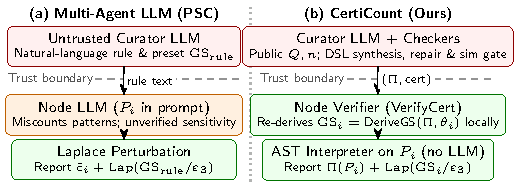
\includegraphics[width=\columnwidth]{figures/fig1_trust_boundary.pdf}
\vspace{-2pt}
\caption{Trust-boundary comparison between (a) multi-agent LLM execution and (b) \textsc{CertiCount}'s certified deterministic execution.}
\label{fig:arch}
\vspace{-4pt}
\end{figure}

\parhead{Graph, Query, and Trust Boundary.}
Let $G=(V,E)$ be an undirected unweighted simple graph with $n=|V|$ nodes $\{0,\dots,n-1\}$. Each node $i \in V$ privately holds its adjacency vector $\mathbf{a}_i \in \{0,1\}^n$, i.e., true neighbor set $P_i = \{j \in V \setminus \{i\} : (i,j) \in E\}$ of degree $d_i = |P_i|$. Given public $n$, budget $\varepsilon > 0$, and natural-language query $Q$, the system estimates target count $f(G)$. As shown in Fig.~\ref{fig:arch}, the curator and aggregator are \emph{untrusted}: they see only public metadata and perturbed transcripts and may issue faulty programs or understated certificates. Each node $i$ runs on a \emph{trusted local server} where $P_i$ never enters an LLM prompt and verification, execution, projection, and noise sampling are local code.

\begin{figure*}[t]
\centering
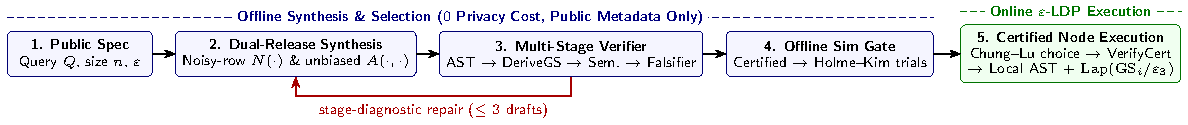
\includegraphics[width=\textwidth]{figures/fig2_pipeline.pdf}
\vspace{-2pt}
\caption{End-to-end \textsc{CertiCount} pipeline: offline verifier-guided synthesis and simulation selection over public inputs (Steps 1--4), followed by online node-verified execution over private neighbor lists (Step 5).}
\label{fig:pipeline}
\vspace{-4pt}
\end{figure*}

\parhead{Node-Level $\varepsilon$-Edge LDP and Budget Split.}
Following~\cite{imola2021locally,zhang2026psc}, $\mathbf{a}_i, \mathbf{a}_i' \in \{0,1\}^n$ are neighboring ($\mathbf{a}_i \sim \mathbf{a}_i'$) if they differ in one bit. Node $i$'s joint transcript $\mathcal{R}_i(\mathbf{a}_i)$ satisfies node-level $\varepsilon$-edge LDP if $\Pr[\mathcal{R}_i(\mathbf{a}_i) \in \mathcal{O}] \le e^{\varepsilon}\Pr[\mathcal{R}_i(\mathbf{a}_i') \in \mathcal{O}]$ for all $\mathbf{a}_i \sim \mathbf{a}_i'$ and measurable $\mathcal{O}$. \textsc{CertiCount} partitions $\varepsilon = \varepsilon_1 + \varepsilon_2 + \varepsilon_3$ (setting unused steps to $0$ and rescaling):\footnote{Under relationship-level accounting---where one undirected edge $(u,v)$ alters both $\mathbf{a}_u$ and $\mathbf{a}_v$ while lower-triangular RR perturbs $(u,v)$ once---the conservative joint budget across transcripts is $\varepsilon_1 + 2\varepsilon_2 + 2\varepsilon_3$ (Sec.~\ref{sec:discussion}).}
(1) \emph{Degree release ($\varepsilon_2$)}: node $i$ publishes $y_i = d_i + \Lap(1/\varepsilon_2)$, yielding per-node edge-clipping bound $D_i = \lfloor \max(y_i, 0) + \alpha \rfloor$~\cite{imola2022communication} ($\alpha \ge 0$) and global $\dhatmax = \min(n-1, \max_j \lfloor \max(y_j, 0) \rfloor)$;
(2) \emph{Edge release ($\varepsilon_1$)}: lower-triangular bits are perturbed by Warner's RR with flip probability $1/(1+e^{\varepsilon_1})$, forming either symmetric $\dhatmax$-projected noisy rows $N(\cdot)$ or the unbiased NAM-DPRD matrix~\cite{guo2025nam} over $D_i$-clipped lists, where $A(j,j)=0$ and for $j \neq k$ with RR bit $\tilde{a}_{jk} \in \{0,1\}$,
\begin{equation}
A(j,k) = \frac{\tilde{a}_{jk}(e^{\varepsilon_1}+1)-1}{e^{\varepsilon_1}-1} \in \Bigl\{-\frac{1}{e^{\varepsilon_1}-1},\, \frac{e^{\varepsilon_1}}{e^{\varepsilon_1}-1}\Bigr\};
\label{eq:nam}
\end{equation}
(3) \emph{Local count ($\varepsilon_3$)}: node $i$ reports $z_i = \Pi(P_i) + \Lap(\GS_i/\varepsilon_3)$ for public post-processing aggregation, where $\GS_i$ is the node-verified sensitivity of Sec.~\ref{sec:cert}. Node-level $(\varepsilon_1+\varepsilon_2+\varepsilon_3)$-edge LDP holds by adaptive sequential composition~\cite{dwork2014algorithmic} under two explicit premises: (P1) the bound $\GS_{\mathrm{own}}$ derived by $\DeriveGS$ satisfies $|\Pi(P_i)-\Pi(P_i')| \le \GS_{\mathrm{own}}$ for all $P_i \sim P_i'$; and (P2) within one run, all \texttt{project} calls at node $i$ share one random vertex order independent of $P_i$.

\section{\textsc{CertiCount} Design}
\label{sec:design}

\subsection{System Overview}
\label{sec:overview}

Fig.~\ref{fig:pipeline} illustrates the workflow. In \emph{offline synthesis} ($0$ privacy budget), the curator LLM runs two repair loops of up to three drafts---one for projected noisy rows $N(\cdot)$, one for the unbiased matrix $A(\cdot,\cdot)$, both also admitting programs over $P$ only. Certified candidates are simulated on public Holme--Kim~\cite{holme2002growing} graphs to discard degenerate estimators and fix the budget split. In \emph{online execution}, if both an $N$- and an $A$-candidate survive with $\varepsilon_2 > 0$, nodes first publish $\{y_i\}$ and the selector picks the release with lower simulated error on Chung--Lu~\cite{chung2002connected} graphs. Each node then runs $\VerifyCert$, executes the AST on $P_i$, and adds $\Lap(\GS_i/\varepsilon_3)$ noise.

\subsection{Graph-LDP DSL and Deterministic Interpreter}
\label{sec:dsl}

\textsc{CertiCount} parses a typed, straight-line Python subset solely via \texttt{ast}: single-assignment lines \texttt{name = expr} ending in \texttt{return expr}, plus a post-processing line \texttt{aggregate: expr} over \texttt{total} ($\sum_i z_i$) and \texttt{n} (clamped at $0$). Expressions have static type \texttt{set}, \texttt{node}, or \texttt{num}:
\begin{itemize}
    \item \textbf{Sets and Nodes:} \texttt{P} ($P_i$, excluding \texttt{self}), \texttt{N(x)} (projected noisy row), \texttt{project(S, k)} ($\le \lfloor k \rfloor$ vertices), and set ops \texttt{\&}, \texttt{|}, \texttt{-}; nodes are \texttt{self} and loop variables.
    \item \textbf{Numbers and Loops:} Public \texttt{D} ($D_i$), \texttt{dmax} ($\dhatmax$), \texttt{n}; \texttt{A(x, y)}; \texttt{size(S)}; \texttt{comb(x, k)} and \texttt{pow(x, k)} (integer constant $k \ge 0$); \texttt{clip(x, lo, hi)}; \texttt{min}/\texttt{max}; \texttt{+}, \texttt{-}, \texttt{*}, \texttt{/} by non-zero public divisors; and bounded sums \texttt{sum(e for j in S)}.
\end{itemize}
Branching, unbounded loops, indexing, private division, and mixing \texttt{N} with \texttt{A} are rejected at parse time:
\begin{lstlisting}[style=dslstyle]
# (a) Noisy-row estimator using RR-projected rows N(j)
Q = project(P, D)  # clip private neighbors to bound D_i
return 0.5 * sum(size(Q & N(j)) for j in Q)  # closed wedges
aggregate: total / 3  # 3 vertices report each triangle

# (b) Matrix estimator using unbiased NAM-DPRD entries A(j, k)
Q = project(P, D)  # coupled random-order projection
return sum(sum(A(j, k) for k in Q) for j in Q)  # A(j,j)=0
aggregate: total / 6  # 6 ordered pairs per triangle
\end{lstlisting}

\parhead{Coupled Random-Order Projection.}
Independent random subsets across multiple \texttt{project} calls can violate replacement sensitivity on nested expressions. To enforce Premise (P2), our coupled operator $\Proj_\pi$ draws a single uniform permutation $\pi$ of $V$ prior to reading $P_i$ and retains the first $\lfloor k \rfloor$ vertices of $S$ under $\pi$. Thus $\Proj_\pi(\Proj_\pi(S, a), b) = \Proj_\pi(S, b)$ for $b \le a$, and $P_i \sim P_i'$ alters $\Proj_\pi(P_i, D_i)$ by at most one vertex swap ($|\cdot \triangle \cdot| \le 2$, size change $\le 1$).

\subsection{Static Sensitivity Derivation and Node Verification}
\label{sec:cert}

Given public parameters $\theta_i = (n, D_i, \dhatmax, \varepsilon_1)$ and graph invariants $\mathcal{F}$ (bounded symmetric rows and irreflexive $P_i$), the static analyzer $\DeriveGS$ propagates abstract bounds over the AST:
\begin{itemize}
    \item \textbf{Set Domain:} Each set $S$ tracks $\sigma(S) = (\mathrm{priv}, s_{\max}, \Delta_{\mathrm{sym}}, \Delta_{\mathrm{size}})$, where the last three entries bound $|S|$, $|S \triangle S'|$, and $\bigl||S|-|S'|\bigr|$ under $P_i \sim P_i'$:
    \begin{equation*}
    \begin{aligned}
    \sigma(\texttt{P}) &= (\mathrm{true},\, n-1,\, 1,\, 1), \\
    \sigma(\texttt{N(x)}) &= (\mathrm{false},\, \min(\dhatmax, n-1),\, 0,\, 0), \\
    \sigma(\texttt{project(S,k)}) &= (\mathrm{priv},\, s',\, \min(2\Delta_{\mathrm{sym}}, 2s'), \\
    &\qquad \min(\Delta_{\mathrm{size}}, s')),
    \end{aligned}
    \end{equation*}
    with $s' = \min(s_{\max}, \lfloor k \rfloor)$ and $\mathrm{priv}, \Delta_{\cdot}$ taken from $\sigma(S)$. Intersecting a private set $S$ with a public set $T$ ($\Delta_{\mathrm{sym}}(T)=0$) tightens the size change to $\lfloor (\Delta_{\mathrm{sym}}(S) + \Delta_{\mathrm{size}}(S))/2 \rfloor$, so $|\texttt{project}(P, D) \cap N(j)|$ changes by at most $1$.
    \item \textbf{Numeric Domain:} Each number tracks $(\mathrm{priv}, \delta, [\ell, u], \mathrm{int})$, refined by three rules.
    (i) \emph{Univariate exact evaluation}: if \texttt{P} enters only via one integer count $X = \texttt{size}(S) \in [\ell, u]$, the analyzer computes $\max_{|x-y|\le \Delta_{\mathrm{size}}(S)} |g(x)-g(y)|$ exactly, giving $\binom{D_i-1}{k-1}$ for \texttt{comb(size(Q), k)} and exact bounds for degree polynomials.
    (ii) \emph{Replacement-coupled sums}: a vertex swap in a sum with public terms in $[\ell, u]$ costs $\max(|\ell|, |u|, u-\ell)$; with $A(j,j)=0$ this gives $2(D_i-1)\bigl(1 + \tfrac{2}{e^{\varepsilon_1}-1}\bigr)$ for matrix triangles.
    (iii) \emph{Row symmetry}: as $\texttt{self} \notin P_i$, \texttt{P \& N(self)} is bounded by $\dhatmax - 1$. Although synthesis rejects own-row reads (Sec.~\ref{sec:selection}), $\VerifyCert$ must certify any program, e.g., PSC reference rules and fuzzed programs.
\end{itemize}

\parhead{Independent Node Verification.}
Given $(\Pi, \mathsf{cert})$ with $\mathsf{cert} = (\mathrm{digest}(\Pi), \theta_i, \mathcal{F}, \GS_{\mathrm{claim}})$, each node runs $\VerifyCert$ to check the SHA-256 digest and $\theta_i$, enforce $\GS_{\mathrm{claim}} \in [0, \infty)$, reject invariants outside its locally enforced set $\mathcal{F}_{\mathrm{local}}$, and recompute $\GS_{\mathrm{own}} = \DeriveGS(\Pi, \theta_i, \mathcal{F}_{\mathrm{local}})$, aborting if $\GS_{\mathrm{claim}} < \GS_{\mathrm{own}}$; otherwise the node calibrates its noise with $\GS_i := \GS_{\mathrm{claim}} \ge \GS_{\mathrm{own}}$.

\begin{proposition}[Conditional Node-Level Edge-LDP]
\label{prop:privacy}
Under Premises (P1)--(P2), for any curator output $(\Pi, \mathsf{cert})$, executing $\Pi$ at node $i$ only after $\VerifyCert$ succeeds satisfies $(\varepsilon_1+\varepsilon_2+\varepsilon_3)$-edge LDP across the full node transcript.
\end{proposition}
\begin{proof}[Proof Sketch]
Degree release $y_i$ satisfies $\varepsilon_2$-LDP ($\GS=1$), with $D_i, \dhatmax$ as post-processing; lower-triangular RR satisfies $\varepsilon_1$-LDP. Conditioned on public transcripts, $\VerifyCert$ ensures $\GS_i \ge \GS_{\mathrm{own}}$ under $\theta_i, \mathcal{F}_{\mathrm{local}}$ (aborting depends only on public inputs). By (P1)--(P2), $|\Pi(P_i) - \Pi(P_i')| \le \GS_{\mathrm{own}} \le \GS_i$, so $\Pi(P_i) + \Lap(\GS_i/\varepsilon_3)$ is $\varepsilon_3$-LDP; adaptive composition completes the claim.
\end{proof}
Premise (P1) rests on manual audit, small-graph falsification, and differential fuzzing (Sec.~\ref{sec:rq2}), rather than mechanized proof.

\begin{table*}[t]
\centering
\caption{Mean relative error $\RE$ ($\downarrow$) across six datasets at $\varepsilon=2$: PSC (Qwen3) ($10$ runs/cell), code baselines GT-PSC and GT-DSL (runs $0..99$), and \textsc{CertiCount} ($20$ designs $\times$ $100$ paired runs; synthesis acceptance $80\%$--$100\%$ per cell).}
\label{tab:rq1}
\scriptsize
\renewcommand{\arraystretch}{1.0}
\setlength{\tabcolsep}{8pt}
\begin{tabular}{ccrrrrrrr}
\toprule
\raisebox{-1.2ex}[0pt][0pt]{Task} & \raisebox{-1.2ex}[0pt][0pt]{Method} & \multicolumn{6}{c}{Datasets} & \raisebox{-1.2ex}[0pt][0pt]{Avg.} \\
\cmidrule(lr){3-8}
 & & \multicolumn{1}{c}{CU} & \multicolumn{1}{c}{Do} & \multicolumn{1}{c}{ML} & \multicolumn{1}{c}{CS} & \multicolumn{1}{c}{EE} & \multicolumn{1}{c}{PM} & \\
\midrule
 & GT-PSC & 0.9386 & 0.8655 & 0.4137 & 1.6135 & 0.4012 & 0.9738 & 0.8677 \\
\raisebox{-1.2ex}[0pt][0pt]{Triangle} & GT-DSL & \textbf{0.5233} & \textbf{0.4185} & \textbf{0.1545} & \textbf{0.8204} & \textbf{0.2625} & \textbf{0.1263} & \textbf{0.3842} \\
 & PSC (Qwen3) & 1.1349 & 1.0827 & 0.8857 & 2.4979 & 0.8934 & \multicolumn{1}{c}{---$^\dagger$} & 1.2989$^\dagger$ \\
 & \textsc{CertiCount} & 0.8537 & 0.6119 & 0.2296 & 1.3722 & 0.2666 & 0.2744 & 0.6014 \\
\midrule
 & GT-PSC & \textbf{0.0216} & \textbf{0.0169} & \textbf{0.0116} & \textbf{0.0249} & \textbf{0.0057} & \textbf{0.0030} & \textbf{0.0140} \\
\raisebox{-1.2ex}[0pt][0pt]{Degree} & GT-DSL & \textbf{0.0216} & \textbf{0.0169} & \textbf{0.0116} & \textbf{0.0249} & \textbf{0.0057} & \textbf{0.0030} & \textbf{0.0140} \\
 & PSC (Qwen3) & 5.4178 & 23.4054 & 2.5344 & 18.4318 & 30.5186 & 104.1606 & 30.7448 \\
 & \textsc{CertiCount} & 0.0219 & 0.0181 & 0.0130 & 0.0253 & 0.0084 & 0.0055 & 0.0154 \\
\midrule
 & GT-PSC & 0.1408 & 0.0863 & 0.0850 & 0.2002 & 0.0499 & 0.0443 & 0.1011 \\
\raisebox{-1.2ex}[0pt][0pt]{2-star} & GT-DSL & \textbf{0.0985} & \textbf{0.0608} & \textbf{0.0388} & \textbf{0.1067} & \textbf{0.0250} & \textbf{0.0074} & \textbf{0.0562} \\
 & PSC (Qwen3) & 0.5816 & 0.4306 & 0.3686 & 0.5081 & 0.4382 & 0.8761 & 0.5339 \\
 & \textsc{CertiCount} & \textbf{0.0985} & \textbf{0.0608} & \textbf{0.0388} & \textbf{0.1067} & \textbf{0.0250} & \textbf{0.0074} & \textbf{0.0562} \\
\midrule
 & GT-PSC & 0.6632 & 0.3125 & 0.2686 & 0.6120 & 0.1918 & 0.1227 & 0.3618 \\
\raisebox{-1.2ex}[0pt][0pt]{3-star} & GT-DSL & \textbf{0.4195} & \textbf{0.1783} & \textbf{0.0645} & \textbf{0.2984} & \textbf{0.0402} & \textbf{0.0087} & \textbf{0.1683} \\
 & PSC (Qwen3) & 1.1591 & 0.6915 & 0.7404 & 0.8065 & 0.8697 & 1.1177 & 0.8975 \\
 & \textsc{CertiCount} & \textbf{0.4195} & \textbf{0.1783} & \textbf{0.0645} & \textbf{0.2984} & \textbf{0.0402} & \textbf{0.0087} & \textbf{0.1683} \\
\bottomrule
\end{tabular}
\par\vspace{2pt}{\centering\scriptsize $^\dagger$PSC (Qwen3) overflows node prompt context on PM Triangle; its Avg.\ spans CU--EE (where \textsc{CertiCount} averages $0.6668$).\par}
\vspace{-4pt}
\end{table*}

\subsection{Noise-Aware Candidate Selection and Iterative Repair}
\label{sec:selection}

Privacy certification alone cannot prevent statistical degeneracy: e.g., a \emph{Triangle-Edge} program summing \texttt{clip(size(Q \& N(j)), 0, 1)} over \texttt{j in Q} passes certification and is exact on noiseless rows, yet RR false edges drive almost every indicator to $1$. Moreover, biased low-$\GS$ rows $N(\cdot)$ and unbiased higher-$\GS$ matrix $A(\cdot,\cdot)$ prevail in different density regimes. \textsc{CertiCount} applies two zero-budget post-processing simulations:
(1) \emph{Design-time gate}: candidates are simulated ($8$ trials/graph) on six public Holme--Kim~\cite{holme2002growing} graphs of size $n$ (degrees $\{4,8,16\} \times$ triad probabilities $\{0.1,0.6\}$), discarding any candidate with geometric-mean $\RE \ge 1.0$ (refusing release if none remain) and fixing the budget split;
(2) \emph{Run-time choice}: if $N$- and $A$-candidates share the chosen split with $\varepsilon_2 > 0$, after publishing $\{y_i\}$ the selector simulates both on three Chung--Lu~\cite{chung2002connected} graphs with expected degrees $\max(y_i, 0)$ before executing $\varepsilon_1$ and $\varepsilon_3$.

\parhead{Verifier-Guided Iterative Repair.}
Each synthesis loop ($\le 3$ drafts) normalizes formatting and executes six ordered deterministic checks:
(1) \emph{Syntax \& Type} (AST validation with syntax hints);
(2) \emph{Deduplication} (canonical digest match);
(3) \emph{Release \& Self-Row} (enforcing $N$- vs.\ $A$-mode separation and rejecting noisy self-lookups \texttt{N(self)} or \texttt{A(self,$\cdot$)} since node $i$ holds exact \texttt{P});
(4) \emph{Sensitivity Tightness} (rejecting an unbounded $\GS$, or one that grows when $n$ is replaced by $4n$ under fixed $D_i, \dhatmax$);
(5) \emph{Noiseless Semantics} (exact match with brute-force counts on $30$ noiseless public graphs); and
(6) \emph{Small-Graph Falsifier} (verifying no edge flip exceeds $\GS$ across all symmetric graphs at $(n=5, \dhatmax=3)$ and $500$ random symmetric graphs at $(n=7, \dhatmax=4)$ over all projection orders).
Upon failure, the base prompt stays fixed and rejected drafts paired with stage-specific diagnostics are appended to a fresh single-turn request.

\section{Evaluation}
\label{sec:eval}

\subsection{Experimental Setup}
\label{sec:setup}

We evaluate six real-world networks from PSC~\cite{zhang2026psc}: Contiguous USA (\texttt{CU}, $n=49$), Dolphins (\texttt{Do}, $62$), Les Mis\'{e}rables (\texttt{ML}, $77$), Ca-sandi\_auths (\texttt{CS}, $86$), Email-Enron-only (\texttt{EE}, $143$), and \emph{C.~elegans} (\texttt{PM}, $453$) at default budget $\varepsilon=2$~\cite{he2025robust,zhang2026psc}. The clipping slack $\alpha=5$ was fixed once by a pilot on \texttt{CU}/\texttt{Do} with expert programs; over $\alpha \in \{0,2,5,10,20\}$ it also minimizes the geometric-mean $\RE$ of expert $k$-star and triangle estimators on the four held-out graphs ($0.080$ vs.\ $0.089$--$0.210$). The curator uses \texttt{Qwen3-8B} (thinking mode, temperature $0.6$). We separate \emph{design repetitions} ($20$ syntheses/cell; $30$ in RQ3) from \emph{noise repetitions} ($100$ runs per accepted design on seeds $0..99$, with code baselines paired on the same seeds), reporting relative error $\RE = |\hat{f} - f| / \max(f, 0.001n)$~\cite{imola2022communication,zhang2026psc}.

In Table~\ref{tab:rq1}, we compare \textsc{CertiCount} against matched-backbone \textbf{PSC (Qwen3)}~\cite{zhang2026psc} (\texttt{Qwen3-8B} curator, \texttt{Qwen3-1.7B} nodes, $10$ runs/cell), \textbf{GT-PSC} (exact Python execution of PSC's DP protocol), and \textbf{GT-DSL} (hand-crafted expert DSL estimators run through \textsc{CertiCount}'s clipping and selection pipeline, i.e., an oracle designer). For unseen subgraph queries (Table~\ref{tab:rq4})---\emph{Open-Wedge} (induced $2$-paths), \emph{High-Degree} (vertices with $d_i \ge 3$), \emph{Triangle-Edge} (edges on $\ge 1$ triangle), and \emph{Triangle-Node} (vertices on $\ge 1$ triangle)---PSC lacks preset rules, so we compare against one-round RR counting (\textbf{GT-Naive}) and \textbf{GT-DSL}. \emph{Triangle} and all unseen queries use a leakage-checked \emph{Zero-Shot Syntax Prompt} containing no benchmark exemplars, whereas single-primitive \emph{Degree} and $k$-star tasks use an earlier \emph{Idiom-Augmented Prompt} with general set-comprehension rewrite idioms.

\subsection{RQ1: Utility, Scalability, and Node Privacy Audit}
\label{sec:rq1}

Table~\ref{tab:rq1} shows that \textsc{CertiCount} lowers average $\RE$ by $1.9\times$ (\emph{Triangle}) to three orders of magnitude (\emph{Degree}) over matched-backbone \textbf{PSC (Qwen3)}, and by $1.4\times$--$2.1\times$ over \textbf{GT-PSC} on $k$-stars and \emph{Triangle}. With $n$, \textsc{CertiCount}'s $\RE$ drops as node noise aggregates at $O(\sqrt{n})$~\cite{imola2021locally}, whereas LLM execution degrades as node prompts lengthen. On \texttt{PM} \emph{Degree}, a same-noise decomposition attributes $0.0033$ $\RE$ to the DP mechanism but over $10^2$ to node-LLM miscounting; on \texttt{PM} \emph{Triangle}, node prompts overflow the context window.

\parhead{Diverse Programs, Identical Estimates.}
A $k$-star query needs only private degrees, whereas \emph{Triangle} must read edges among neighbors via $N(\cdot)$ or $A(\cdot,\cdot)$. On $k$-stars, \textsc{CertiCount} equals \textbf{GT-DSL} although the LLM rarely copies the expert: the $119$ accepted 3-star designs span $53$ distinct programs, only $23$ verbatim equal to the expert \texttt{return comb(size(project(P, D)), 3)}; others write, e.g., \texttt{d = size(project(P, D))} then \texttt{return d*(d-1)*(d-2)/6}. All compute the same clipped count with the same derived $\GS$ and budget split, and paired runs share seeds, clipping bounds, and projection orders, so every estimate coincides (2-star: $45$ distinct among $116$). On \emph{Triangle}, none of $110$ accepted designs ($86$ distinct) copies the expert, yet $80$ reproduce its matrix estimate in every run, e.g., \texttt{sum(sum(A(u,v) for v in S) for u in S)/2} with \texttt{total/3} versus the expert's undivided sum with \texttt{total/6}. The gap to \textbf{GT-DSL} ($0.60$ vs.\ $0.38$) stems from release coverage, not program text: $73$ designs certify only a matrix program and cannot switch to noisy rows on \texttt{CU}/\texttt{Do}, and a few RR-biased designs inflate \texttt{PM} error.

\parhead{Empirical Privacy Audit and Attribution.}
Black-box node execution also breaks nominal LDP guarantees. Auditing node reports on \texttt{PM} \emph{Degree} ($\GS=1, \varepsilon_3=2$) via Bonferroni-corrected Clopper--Pearson lower bounds~\cite{jagielski2020auditing} ($300$--$500$ trials/side) over $60$ degree-stratified nodes confirms empirical $\varepsilon_3$ violations on $31/60$ nodes for \texttt{Qwen3-1.7B} and $15/60$ for \texttt{Qwen3-8B} ($7/60$ and $4/60$ on random-index controls). \textsc{CertiCount}'s interpreter shows $0/20$ on the nodes and pairs where \texttt{Qwen3-8B} violated. The $k$-star gains over \textbf{GT-PSC} stem from per-node edge clipping~\cite{imola2022communication}, which tightens $\binom{D_i-1}{k-1}$ for low-degree nodes.

\subsection{RQ2: Certification Soundness and Simulation Selection}
\label{sec:rq2}

\begin{table}[t]
\centering
\caption{Certification counterfactuals, fuzzing, and fault injection.}
\label{tab:rq2}
\scriptsize
\setlength{\tabcolsep}{3pt}
\begin{tabular}{lrrc}
\toprule
Evaluation suite & Volume & Viol.\ w/o cert. & Unsound \\
\midrule
Counterfactual replay$^\dagger$ & 201 runnable & 107 (53.2\%) & \textbf{0} \\
End-to-end synthesis campaigns & 2,471 drafts & 752 & \textbf{0} \\
Differential fuzzing ($N$, $A$, node) & 16,000 progs & --- & \textbf{0} \\
Node certificate fault injection & 104,904 checks & --- & \textbf{0} \\
\bottomrule
\end{tabular}
\par\vspace{2pt}{\raggedright\scriptsize Viol.\ w/o cert.: runnable drafts exceeding the preset reference $\GS$ when run without $\DeriveGS$; Unsound: refuted derived bounds or accepted tampered certificates. $^\dagger$Full-transcript subset on Triangle and Open-Wedge ($302$ drafts, $201$ runnable); worst-case loss $\ge 28.7\varepsilon_3$.\par}
\vspace{-2pt}
\end{table}

\begin{table*}[t]
\centering
\caption{Mean relative error $\RE$ ($\downarrow$) on unseen subgraph queries under the Zero-Shot Syntax Prompt ($\varepsilon=2$, $20$ designs $\times$ $100$ runs/cell paired on seeds $0..99$).}
\label{tab:rq4}
\scriptsize
\renewcommand{\arraystretch}{1.0}
\setlength{\tabcolsep}{8pt}
\begin{tabular}{ccrrrrrrr}
\toprule
\raisebox{-1.2ex}[0pt][0pt]{Task} & \raisebox{-1.2ex}[0pt][0pt]{Method} & \multicolumn{6}{c}{Datasets} & \raisebox{-1.2ex}[0pt][0pt]{Avg.} \\
\cmidrule(lr){3-8}
 & & \multicolumn{1}{c}{CU} & \multicolumn{1}{c}{Do} & \multicolumn{1}{c}{ML} & \multicolumn{1}{c}{CS} & \multicolumn{1}{c}{EE} & \multicolumn{1}{c}{PM} & \\
\midrule
 & GT-Naive & 5.1291 & 3.8197 & 3.2747 & 15.3323 & 5.8313 & 9.6771 & 7.1773 \\
Open-Wedge & GT-DSL & \textbf{0.3755} & \textbf{0.2346} & \textbf{0.1590} & \textbf{0.3791} & 0.1812 & 0.0297 & \textbf{0.2265} \\
 & \textsc{CertiCount} & 0.7410 & 0.4184 & 0.3038 & 0.7182 & \textbf{0.1739} & \textbf{0.0292} & 0.3974 \\
\midrule
 & GT-Naive & 0.1370 & 0.3187 & 0.5392 & 1.4566 & 0.1818 & 0.0486 & 0.4470 \\
High-Degree & GT-DSL & 0.1077 & 0.1143 & 0.1179 & \textbf{0.1763} & \textbf{0.0585} & \textbf{0.0281} & \textbf{0.1005} \\
 & \textsc{CertiCount} & \textbf{0.1075} & \textbf{0.1139} & \textbf{0.1175} & 0.1766 & 0.0602 & 0.0292 & 0.1008 \\
\midrule
 & GT-Naive & 0.8628 & 1.5600 & 1.1836 & 4.2415 & 1.8475 & 5.8524 & 2.5913 \\
Triangle-Edge & GT-DSL & \textbf{0.4892} & \textbf{0.4833} & 0.4079 & \textbf{0.6340} & \textbf{0.2258} & \textbf{0.1821} & \textbf{0.4037} \\
 & \textsc{CertiCount} & 0.4986 & 0.5648 & \textbf{0.3739} & 0.7128 & 0.2739 & 0.1912 & 0.4359 \\
\midrule
 & GT-Naive & \textbf{0.0144} & 0.3354 & 0.3451 & 0.5833 & \textbf{0.1000} & \textbf{0.0203} & 0.2331 \\
Triangle-Node & GT-DSL & 0.2017 & \textbf{0.2203} & 0.2322 & \textbf{0.2411} & 0.1173 & 0.0756 & \textbf{0.1814} \\
 & \textsc{CertiCount} & 0.2167 & 0.2408 & \textbf{0.2085} & 0.2692 & 0.1336 & 0.0743 & 0.1905 \\
\bottomrule
\end{tabular}
\vspace{-4pt}
\end{table*}

Table~\ref{tab:rq2} shows why static certification is indispensable under an untrusted curator. Replayed under the preset reference sensitivity without $\DeriveGS$, over half of runnable LLM drafts violate the nominal $\GS$, with worst-case local privacy loss above $28\varepsilon_3$. By contrast, small-graph falsification refutes \emph{zero} $\DeriveGS$ bounds across all $2{,}471$ synthesized drafts and $16{,}000$ fuzzed noisy-row, matrix, and per-node programs, and $104{,}904$ tampered-certificate checks yield zero unsafe acceptances at $0.03$\,ms median node latency. Simulation also governs utility: on \texttt{PM} \emph{Triangle} (exemplar-bearing prompt), replacing a noiseless threshold gate with Holme--Kim simulation raises acceptance from $60\%$ to $100\%$ and cuts $\RE$ from $1.182$ to $0.197$. Chung--Lu run-time selection improves over design-time-only selection (e.g., \texttt{CS} \emph{Triangle} $1.477 \to 0.873$) but misses the better release on \texttt{EE} \emph{Triangle} ($0.239$ vs.\ $0.124$).

\subsection{RQ3: Role of Diagnostic Feedback in Iterative Synthesis}
\label{sec:rq3}

\begin{figure}[t]
\centering
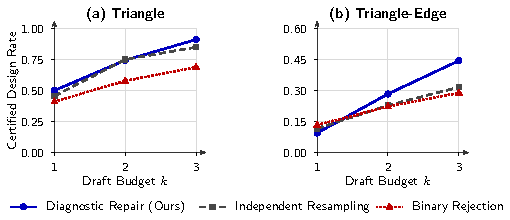
\includegraphics[width=\columnwidth]{figures/fig3_diagnostic_repair.pdf}
\vspace{-2pt}
\caption{Cumulative certified design rate across draft budgets $k \in \{1,2,3\}$ ($30$ designs/cell; Diagnostic Repair and Independent Resampling pooled over six networks, Binary Rejection over \texttt{CU}, \texttt{EE}, \texttt{ML}).}
\label{fig:feedback}
\vspace{-4pt}
\end{figure}

We compare three variants with identical first-draft prompts ($30$ designs/cell, $\le 3$ drafts/release) on \emph{Triangle} and \emph{Triangle-Edge}: \textbf{Diagnostic Repair} (rejected drafts + stage-specific diagnostics), \textbf{Binary Rejection} (rejected drafts + bare ``rejected''), and \textbf{Independent Resampling} (no history). First-draft rates are comparable across arms (within $9$ points; Fig.~\ref{fig:feedback}). Pooled over six networks ($360$ designs/arm), \textbf{Diagnostic Repair} raises certified yield over \textbf{Independent Resampling} by $9.2$ points ($243$ vs.\ $210$; Cochran--Mantel--Haenszel $p = 0.0039$), mainly on \emph{Triangle-Edge} ($+12.2$, $p = 0.023$; \emph{Triangle}: $+6.1$, $p = 0.10$), and cuts LLM calls per published estimator by $15\%$ ($28\%$ on \emph{Triangle-Edge}). On \texttt{CU}, \texttt{EE}, \texttt{ML} ($180$ designs/arm), \textbf{Binary Rejection} trails \textbf{Diagnostic Repair} by $18.3$ points ($p = 1.5\times 10^{-4}$) and does not beat resampling ($-8.3$, $p = 0.094$; $-15.6$, $p = 0.023$ on \emph{Triangle}), as bare rejections anchor the LLM onto near-duplicate rewrites. After Self-Row and Sensitivity Tightness rejections on \emph{Triangle}, $73\%$--$86\%$ of diagnostic next drafts pass the failed stage, versus $28\%$--$44\%$ under resampling.

\subsection{RQ4: Generalization to Unseen Subgraph Queries}
\label{sec:rq4}

Table~\ref{tab:rq4} evaluates zero-shot generalization to four unseen queries. On \emph{Open-Wedge}, \emph{High-Degree}, and \emph{Triangle-Edge}, \textsc{CertiCount} outperforms \textbf{GT-Naive} on every dataset (Avg.\ $\RE$ $4.4\times$--$18.1\times$ lower) and tracks hand-crafted \textbf{GT-DSL}, nearly matching it on \emph{High-Degree}. On \emph{Triangle-Edge}, nested indicator clipping lowers acceptance to $35\%$--$55\%$. On \emph{Triangle-Node}, \textsc{CertiCount} lowers Avg.\ $\RE$ but trails \textbf{GT-Naive} on \texttt{CU}, \texttt{EE}, \texttt{PM}, where $91\%$--$98\%$ of vertices lie on triangles, so dense RR graphs trivially report $\approx n$.

\section{Discussion and Limitations}
\label{sec:discussion}

\parhead{Mechanized Proof and Privacy Granularity.}
Despite zero refutations across $2{,}471$ drafts and $16{,}000$ fuzzed programs, Premise (P1) lacks mechanized verification. Following~\cite{imola2021locally,zhang2026psc}, we adopt node-level $\varepsilon$-edge LDP; protecting an edge across both endpoints' transcripts requires relationship-level accounting $\varepsilon_1 + 2\varepsilon_2 + 2\varepsilon_3$ (halving $\varepsilon_2$ and $\varepsilon_3$).

\parhead{Scope and Automation Value.}
Experiments focus on $\varepsilon=2$ and Qwen3 backbones, with the Idiom-Augmented Prompt on \emph{Degree}/$k$-stars and the Zero-Shot Syntax Prompt elsewhere. $k$-stars admit one canonical estimator, so matching \textbf{GT-DSL} there shows reliability rather than design ingenuity; the value of \textsc{CertiCount} lies in automating certified synthesis without per-query expert derivations. Queries with sensitivity $O(D_i \dhatmax)$ (e.g., $4$-cycles) remain noise-bound and are refused by the simulation gate.

\parhead{Cooperation Model.}
\textsc{CertiCount} replaces trust between parties with verifiable artifacts: the curator contributes design effort but no authority, and each node accepts work only after re-derivation. The same contract fits institutions jointly counting patterns over a shared contact graph without running each other's unchecked code.

\section{Conclusion}
\label{sec:conclusion}

We presented \textsc{CertiCount}, decoupling LLM-based estimator synthesis from certified deterministic node execution under $\varepsilon$-edge LDP, so that untrusted designers and data owners cooperate through checkable programs and certificates. Combining public-metadata DSL synthesis, diagnostic repair, node-re-derived sensitivity certificates, and zero-budget simulation selection eliminates node-LLM counting errors, context overflow, and empirical privacy violations while generalizing to unseen subgraph queries.

\bibliographystyle{IEEEtran}
\bibliography{references}

\end{document}
